\documentclass[11pt]{article}
\usepackage{spikey}
\usepackage{amsmath}
\usepackage{amssymb}
\usepackage{soul}
\usepackage{float}
\usepackage{graphicx}
\usepackage{subfig}
\usepackage{hyperref}
\usepackage{xcolor}
\usepackage{chngcntr}
\usepackage{centernot}
\usepackage{datetime}
\usepackage[shortlabels]{enumitem}

\usepackage[margin=1truein]{geometry}
\usepackage{setspace}
\linespread{1.15}

\counterwithin{equation}{section}
\newcommand{\upi}[0]{^{(i)}}

\title{CS229 Problem Set 2}
\date{\today}
\author{Tianyu Du}
\begin{document}
	\maketitle
	\newpage
	\section{Problem 1 Logistic Regression: Training Stability}
	\subsection{1(a)}
	\paragraph{Comment} The parameter trained on dataset A converges after around 30,000 iterations of gradient ascent. In contrast, on dataset B, the training algorithm does not reach convergence within a reasonable amount of time.
	\newpage
	\subsection{1(b)}
	\begin{figure}[h]
	    \centering
	    \subfloat[Dataset A]{{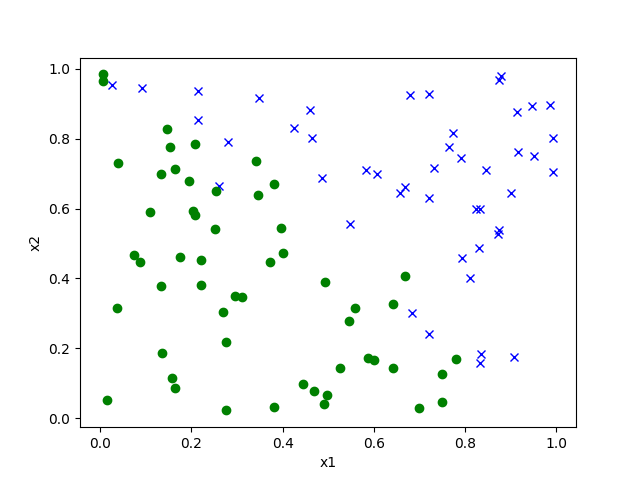
\includegraphics[width=0.5\linewidth]{./src/stability/ds1_a.png}}}
	    \subfloat[Dataset B]{{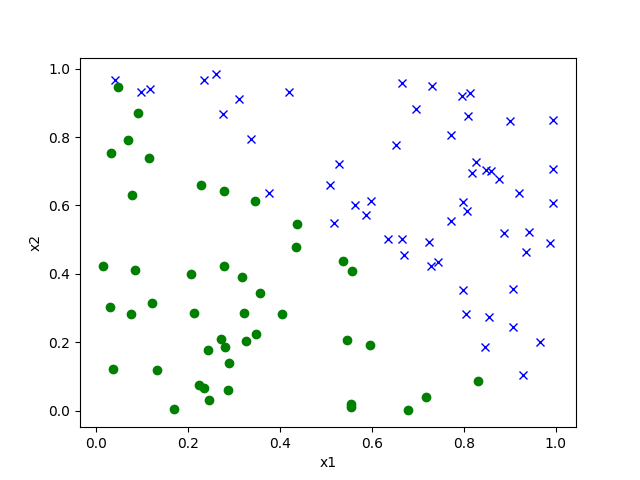
\includegraphics[width=0.5\linewidth]{./src/stability/ds1_b.png}}}
	    \caption{Two Datasets}
	\end{figure}
	\paragraph{Comment} From the plot of two datasets we can see that dataset B is more \emph{linearly separable} than dataset A. There exists intermixing of data points belonging to both classes in dataset A, but fewer can be observed in dataset B. The linear separability of dataset B causes the instability of logistic regression on it. In the scenario of dataset B, we claim that the gradient descent algorithm increases $\theta$ indefinitely without convergence.
	\begin{proof}
		Let $\mc{A}$ and $\mc{B}$ denote two datasets respectively.
%		The gradient descent for logistic regression works as
%		\begin{align}
%			\theta \leftarrow \theta + \alpha \sum_{i=1}^n \left(y\upi - h_\theta(x\upi)\right) x\upi
%		\end{align}
		And the log-likelihood looks like
		\begin{align}
			\ell (\theta) &= \sum_{i=1}^{n} y^{(i)} \log h_\theta\left(x^{(i)}\right)+\left(1-y^{(i)}\right) \log \left(1-h_\theta\left(x^{(i)}\right)\right) \\
			&= \underbrace{\sum_{i: y\upi = 0} \log \left(1 - h_\theta(x\upi)\right)}_{P} + 
			\underbrace{\sum_{i: y\upi = 1} \log h_\theta(x\upi)}_{Q}
		\end{align}
		Suppose the threshold for classification is 0.5, and dataset $\mc{B}$ can be separated perfectly with some $\theta \in \R^d$. That's, for (almost) every sample $i \in \mc{B}$ such that $y\upi = 0$, $\theta^T x\upi < 0$ and for (almost) every $y\upi = 1$, $\theta^T x\upi > 0$. As a result, for every $\theta^t$ that separate dataset $\mc{B}$ almost perfectly, suppose $\theta^t$ is inflated to $\theta^{t+1} := (1 + \varepsilon) \theta^t$ for some $\varepsilon > 0$, for those negative samples ($y\upi = 0$), $\theta^T x\upi$ changes to $(1 + \varepsilon) \theta^T x\upi < \theta^T x\upi < 0$, and $h_\theta(x\upi)$ decreases. As a result, $P$ increases. Similarly, for those positive samples, $\theta^T x\upi$ changes to $(1 + \varepsilon) \theta^T x\upi > \theta^T x\upi > 0$, and $h_\theta(x\upi)$, so does $Q$.\\
		It is shown that for each $\theta^t$ separates dataset perfectly (or at least almost perfectly, because if the misclassified group is small, we can safely ignore the contribution to likelihood function from samples from the misclassified group), the log likelihood is increased when $\theta$ is inflated, and the resulted $\theta^{t+1}$ is still a (almost) perfect-separating parameter. Also, there is no upper bound on $\norm{\theta}$, therefore, the gradient ascend algorithm will run indefinitely to increase $\ell(\theta)$ by inflation the norm of $\theta$.\\
		For dataset like $\mc{A}$, for each $\theta$, the misclassified group provides significant contributions to $\ell(\theta)$, inflating $\theta$ comes with the cost of reduced likelihood on samples from the misclassified groups. By the nature of $\log$ function, the cost of likelihood reduction on misclassified group will eventually overcome the the likelihood gain by expanding $\theta$, and $\ell(\theta)$ cannot be risen to infinity on this kind of datasets. Therefore, the algorithm stops at some $\theta^*$.
	\end{proof}
	\newpage
	\subsection{1(c)}
		\paragraph{Comment}
		\begin{enumerate}[(i)]
			\item (NO) A different constant learning rate won't help because the $\nabla_\theta \ell(\theta)$ does not vanish, and the update step $\alpha \nabla_\theta \ell(\theta)$ is always significant. Therefore, convergence is still not achievable.
			\item (NO) Annealing the learning rate will not mitigate the problem because this does not change the fact that the maximum of $\ell$ is achieved when $\theta \to \infty$.
			\item (NO) Linear scaling does not change the fact that dataset is well (linearly) separable, $\theta$ is still going to explode indefinitely.
			\item (YES) Adding regularization helps. As mentioned before, the main cause of interminability of gradient ascent is $\ell(\theta)$ can always be increased by inflating $\theta$ (i.e. increasing $\norm{\theta}$). The regularizing term prevents $\theta$ from exploding and enforce the convergence.
			\item (YES) Give the variance of noise is large enough, the noise helps eliminate the linear separability of data, so that the dataset becomes intermixing.
		\end{enumerate}
	
	\newpage
	\subsection{1(d)}
	\paragraph{Comment} SVM is more robust against linearly separable dataset. SVM is seeking to construct a hyperplane $w^T x + b$ to maximize the geometric margin $\gamma$, while controlling $\norm{w} = 1$. Note that changing $b$ would shift the position of the hyperplane, therefore at optimal, $b^* < \infty$. Also, the performance measure of SVM using geometric margin is invariant to scales of $(w, b)$. Therefore, given the constraint on $\norm{w}$, SVM using geometric margin does not suffer from the parameter exploding problem (optimal is achieved when $\theta \to \infty$), and the optimal $(w^*, b^*)$ will both be finite.
	
	\newpage
	\section{Problem 2 Spam Classification}
	\subsection{2(a)}
	\paragraph{Result} \texttt{Size of dictionary: 1722}
	
	\newpage
	\subsection{2(b)}
	\paragraph{Result} \texttt{Naive Bayes had an accuracy of 0.978494623655914 on the testing set}
	
	\newpage
	\subsection{2(c)}
	\paragraph{Result} \texttt{The top 5 indicative words for Naive Bayes are:  ['claim', 'won', 'prize', 'tone', 'urgent!']}
	
	\newpage
	\subsection{2(d)}
	\paragraph{Result} \texttt{The optimal SVM radius was 0.1}
	
	\newpage
	\section{Problem 4 Kernelizing the Perceptron}
	\subsection{4(a)}
	\paragraph{Answer} The kernel trick firstly represents each $\theta\upi$ as a linear combination of features of observations:
	\begin{align}
		\theta\upi = \sum_{\ell=1}^n \beta_\ell\upi \phi(x^{(\ell)})
	\end{align}
	$\theta^{(0)}$ can be represented simply by setting $\beta_\ell^{(0)} = 0$ for every $\ell$. To make prediction, $\theta\upi \cdot \phi(x^{(i+1)})$ is firstly computed as 
	\begin{align}
		\theta\upi \cdot \phi(x^{(i+1)}) &= \left[ \sum_{\ell=1}^n \beta_\ell\upi \phi(x^{(\ell)})\right] \cdot \phi(x^{(i+1)}) \\
		&= \sum_{\ell=1}^n \left[ \beta_\ell\upi \phi(x^{(\ell)}) \cdot \phi(x^{(i+1)}) \right] \\
		&= \sum_{\ell=1}^n \beta_\ell\upi K \left(\phi(x^{(\ell)}),\phi(x^{(i+1)}) \right) \\
	\end{align}
	The prediction is given by 
	\begin{align}
		h_{\theta\upi}(x^{(i+1)}) &= \tx{sign} \left (
			\sum_{\ell=1}^n \beta_\ell\upi K \left(\phi(x^{(\ell)}),\phi(x^{(i+1)}) \right)
		\right )
	\end{align}
	According to the given update rule, 
	\begin{align}
		\theta^{(i+1)} &= \sum_{\ell=1}^n \beta_\ell^{(i+1)} \phi(x^{(\ell)}) \\
		&:= \theta\upi + \alpha \left(y^{(i+1)} - h_{\theta\upi}(x^{(i+1)})\right) \phi(x^{(i+1)}) \\
		&= \sum_{\ell=1}^n \beta_\ell^{(i)} \phi(x^{(\ell)}) 
		+ \alpha \left(y^{(i+1)} - h_{\theta\upi}(x^{(i+1)})\right) \phi(x^{(i+1)})
	\end{align}
	Note that at this epoch, only $\beta_{i+1}$ is modified,
	\begin{align}
		\beta_{i+1}^{(i+1)} &:= \beta_{i+1}\upi + \alpha \left(y^{(i+1)} - h_{\theta\upi}(x^{(i+1)})\right) \\
		&= \beta_{i+1}\upi +\alpha \left(y^{(i+1)} - g(\theta\upi \cdot \phi(x^{(i+1)}) )\right)
	\end{align}
	For any $\ell \neq i + 1$,
	\begin{align}
		\beta_{\ell}^{(i+1)} := \beta_{\ell}^{(i)}
	\end{align}
	Given that $\beta^{(0)}_\ell$s are initialized to zero. And $\beta_{\ell}$ is updated at and only at step $\ell$. Therefore, $\beta_{i+1}\upi = \beta_{i+1}^{(0)} = 0$. The update rule can also be written as
	\begin{align}
		\beta_{i+1}^{(i+1)} &:= \alpha \left(y^{(i+1)} - g(\theta\upi \cdot \phi(x^{(i+1)}) )\right)
	\end{align}
\end{document}



















